
\section{Difusión con reacción química homogénea}

\begin{minipage}{0.5\textwidth} 
    \centering
    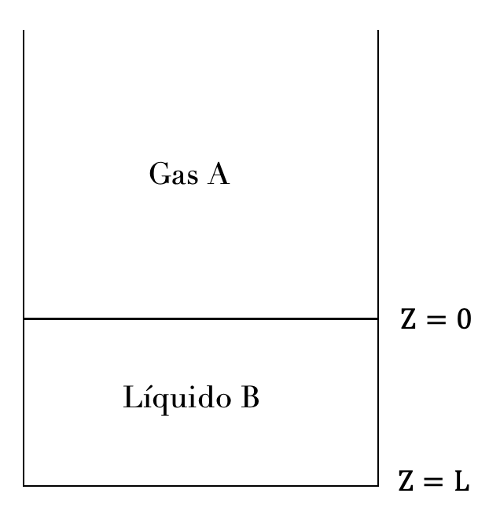
\includegraphics[width=0.8\linewidth]{Capitulo2/Imagenes/Fig_2.9.png} 
    \captionof{figure}{Absorción de A en B con reacción homogénea en la fase líquida} 
    \label{fig:Fig_2.9}
\end{minipage}%
\begin{minipage}{0.4\textwidth} 
    En la figura \textbf{\eqref{fig:Fig_2.9}}, el gas \( A \) se disuelve en el líquido \( B \). Al difundirse \( A \) en \( B \), ocurre una reacción \( A + B \xrightarrow{} AB \). Por ejemplo, la absorción de \( CO_2 \) en una solución de NaOH.
        En este caso, el proceso es descrito por la ecuación \textbf{\eqref{eq_1.30}}, en la cual, no hay dependencia con el tiempo y el sistema está en reposo \( \underline{v} = 0 \).
\end{minipage}
    

\vspace{1 cm}
Suponiendo una reacción de primer orden para la descomposición de A, la ecuación \textbf{\eqref{eq_1.30}} se reduce a:

\begin{equation}   
 \mathscr{D}_{AB}\frac{d^2(C_A)}{dz^2}+R_A=0
 \label{eq_2.55}
\end{equation}


En donde:\begin{equation}
    R_A=\frac{d(C_A)}{dt}=-kC_A
    \label{eq_2.56}
\end{equation}
Este sistema otorga las siguientes condiciones de frontera:

\begin{equation}
    C_A|_{z=0} = C_{A0}, \quad \frac{d(C_A)}{dz}\bigg|_{z=L} = N_{Az}|_{z=L} = 0
    \label{eq_2.57}
\end{equation}

Se definen las siguientes variables adimensionales: $\Gamma=\frac{C_A}{C_{A0}}$ y $\zeta=\frac{z}{L}$

La ecuación \eqref{eq_2.55} se transforma en:
\begin{equation}
    \frac{d^2\Gamma}{d\zeta^2}-\left(\frac{k_1L^2}{\mathscr{D}_{AB}}\right)\Gamma=0
    \label{eq_2.58}
\end{equation}
\quad donde
\begin{equation}
  \phi=\left( \frac{k_1L^2}{\mathscr{D}_{AB}}\right)^{1/2}
\end{equation}

es el módulo de Thiele. \\Las condiciones de frontera adimensionales son ahora:
\begin{equation}
 \Gamma|_{\zeta=0}=1   
\quad \text{y} \quad
 \frac{d\Gamma}{d\zeta}|_{\zeta=1}=0   
 \label{eq_2.60}
\end{equation}

La solución de la ecuación \eqref{eq_2.58} corresponde a:
\begin{equation}
    \Gamma=C_1\cosh({\phi\zeta})+C_2\sinh({\phi\zeta})
    \label{eq_2.61}
\end{equation}
Aplicando \eqref{eq_2.61} obtenemos $C_1$ y $C_2$:

 $C_1=1$ y $0=\phi \sinh({\phi})+C_2\phi \cosh(\phi)\longrightarrow C_2=-\frac{\sinh(\phi)}{\cosh({\phi})}=-\tanh({\phi})$
La ec. \eqref{eq_2.60} tiene la siguiente solución particular:
 \begin{equation}
  \Gamma=\frac{\cosh[{\phi(1-\zeta)}]}{\cosh({\phi})}   
  \label{eq_2.62}
 \end{equation}

La concentración promedio de A en la fase líquida es;

 \begin{equation}
     \overline{\Gamma}=\frac{\int_0^1\Gamma d\zeta}{\int_0^1d\zeta}=\frac{1}{\cosh(\phi)}\left[\frac{\sinh[\phi(1-\zeta)]_{0}^1}{-\phi}\right]=\frac{\tanh(\phi)}{\phi}
     \label{eq_2.63}
 \end{equation}
 
El flux molar en $z=0$ es:

\begin{equation}
    N_{Az}|_{z=0}=-\mathscr{D}_{AB}\frac{d(C_A)}{dz}|_{z=0}=-\mathscr{D}_{AB}\frac{C_{A0}}{L}\frac{d\Gamma}{d\zeta}|_{\zeta=0}=\mathscr{D}_{AB}\frac{C_{A0}}{L}\phi\tanh(\phi)
\end{equation}



\subsection{Absorción de gas con reacción química en un tanque de agitación}
Considere un sistema en el que el gas A disuelto se combina con el líquido B por una reacción química de primer orden. Por ejemplo, la absorsión de $SO_2$ o $H_2S$ en NaOH en solución acuosa.

\begin{figure}[H]
    \centering
    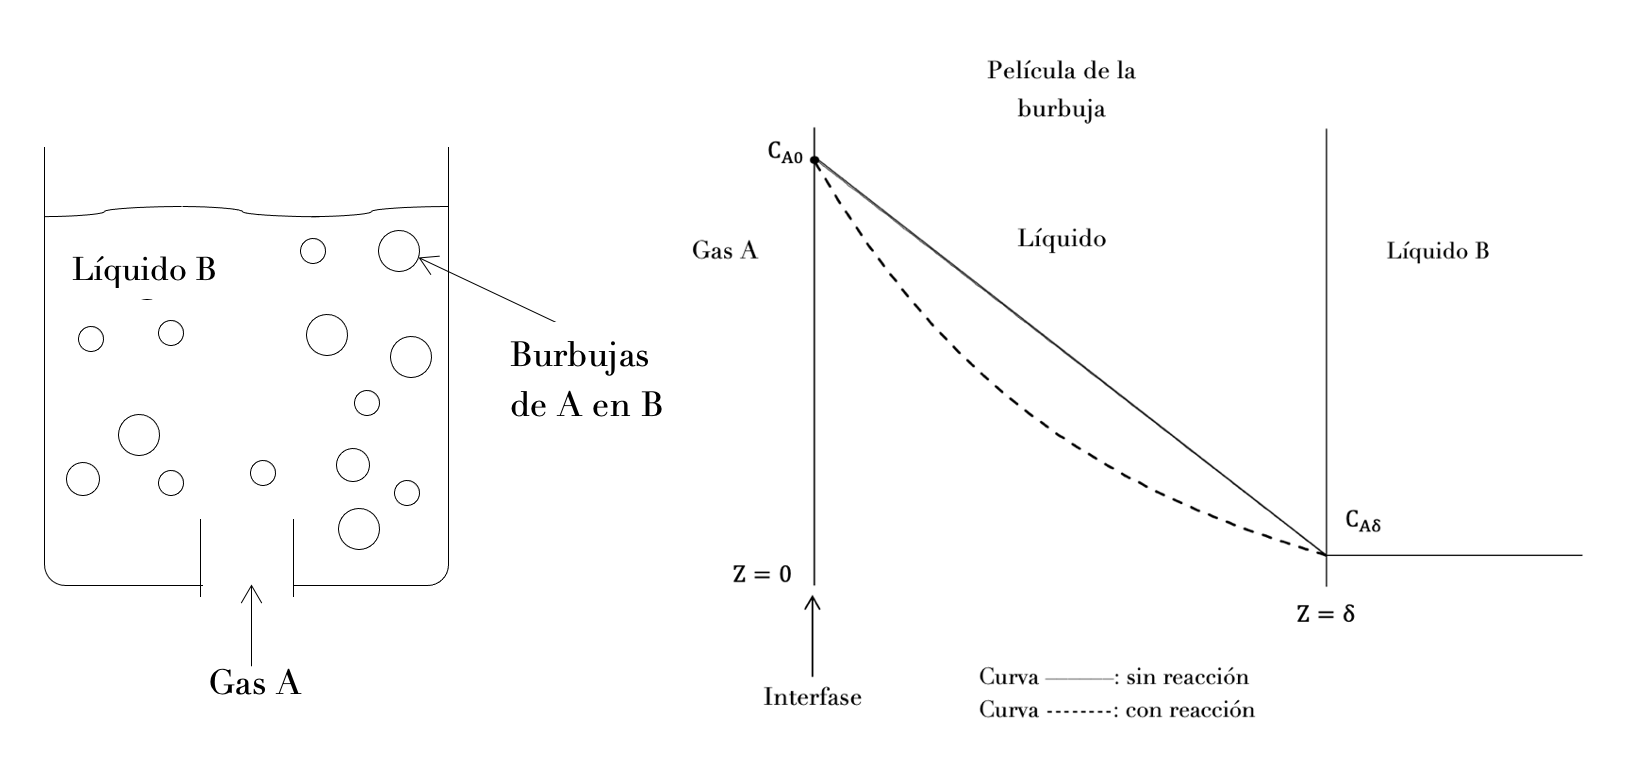
\includegraphics[width=\linewidth]{Capitulo2/Imagenes/Fig_2.10.png}
    \caption{Perfil de concentración predicho en la película de líquido que rodea a una burbuja}
    \label{fig:fig_2.10}
\end{figure}

Condiciones de forntera:
\begin{equation}
    C_A|_{z=0}=C_{A0} \quad\text{y}\quad
    C_A|_{z=\delta}=C_{A\delta}
\end{equation}
O en variables adimensionales:
\begin{equation}
    \Gamma|_{\zeta=0}=1 \quad \text{y} \quad
    \Gamma|_{\zeta=1}=B
        \label{eq_2.66}
\end{equation}
En donde 
\begin{equation*}
    \zeta = \frac{z}{\delta}, \quad \Gamma = \frac{C_A}{C_{A0}}, \quad B = \frac{C_{A\delta}}{C_{A0}}, \quad \phi^2 = \frac{k_1 \delta^2}{\mathscr{D}_{AB}}
\end{equation*}


La ecuación \eqref{eq_2.61} con las condiciones \eqref{eq_2.66} tiene la siguiente solución:

\begin{equation}
    \Gamma=\frac{\sinh(\phi)\cosh(\phi\zeta)+(B-\cosh(\phi))\sinh(\phi\zeta)}{\sinh(\phi)}
    \label{eq_2.67}
\end{equation}
La ecuación \eqref{eq_2.67} describe el perfil de la curva con reacción. Se supone que la concentración de A fuera de la película es $C_{A\delta}$, por lo que, si la superficie de todas las burbujas en la superficie es S, la cantidad de A consumida por la reacción química es:

\begin{equation}
    SN_{Az}|_{z=\delta}=-S\mathscr{D}_{AB}\frac{dC_A}{dz}|_{z=\delta}=Vk_1C_A\delta
    \label{eq_2.68}
\end{equation}
En donde V es el volumen de la fase líquida.
Luego:

\begin{equation*}
    -\frac{dC_A}{dz}|_{z=\delta}=-\frac{C_{A0}}{\delta}\frac{d\Gamma}{d\zeta}|_{\zeta=1}=\frac{Vk_1C_{A\delta}}{S\mathscr{D}_{AB}}\longrightarrow-\frac{d\Gamma}{d\zeta}|_{\zeta=1}=\frac{V}{S\delta}\phi^2B
\end{equation*}
Como $\cosh^2(\phi)-\sinh^2(\phi)=1$, de la ec. \eqref{eq_2.67} se obtiene:

\begin{equation*}
    \frac{B\cosh(\phi)-1}{\sinh(\phi)}=-\frac{V}{S\delta}B\phi\longrightarrow B(\cosh(\phi)+\frac{V}{S\delta}\phi\sinh(\phi))=1
\end{equation*}
Substituyendo B en la solución para Gamma \eqref{eq_2.67}, obtenemos:
\begin{equation}
    \Gamma=\frac{\cosh(\phi)\cosh(\phi\zeta)-\cosh(\phi)\sinh(\phi\zeta)}{\sinh(\phi)}+\frac{\sinh(\phi)\zeta}{\sinh(\phi)}[\frac{1}{\cosh(\phi)+\frac{V\phi\sinh(\phi)}{S\delta}}]
    \label{eq_2.69}
\end{equation}
El flux de masa absorbido con reacción química ( normalizada) es:

\begin{equation}
\begin{split}
    \widetilde{N} &= \frac{N_{Az}}{\mathscr{D}_{AB}\frac{C_{A0}}{\delta}} = -\frac{\mathscr{D}_{AB}}{\mathscr{D}_{AB}\frac{C_{A0}}{\delta}} \frac{d(C_A)}{dz}\bigg|_{z=0} \\
    &\Rightarrow -\frac{d\Gamma}{d\zeta}\bigg|_{\zeta=0} = \frac{\phi \cosh(\phi)}{\sinh(\phi)} - \frac{\phi}{\sinh(\phi)\left(\cosh(\phi) + \frac{V\phi \sinh(\phi)}{S\delta}\right)} \\
    &= \frac{\phi}{\sinh(\phi)}\left[\cosh(\phi) - \frac{1}{\cosh(\phi) + \frac{V}{S\delta}\phi \sinh{\phi}}\right]
\end{split}
\label{eq_2.70}
\end{equation}

\begin{figure}[H]
    \centering
    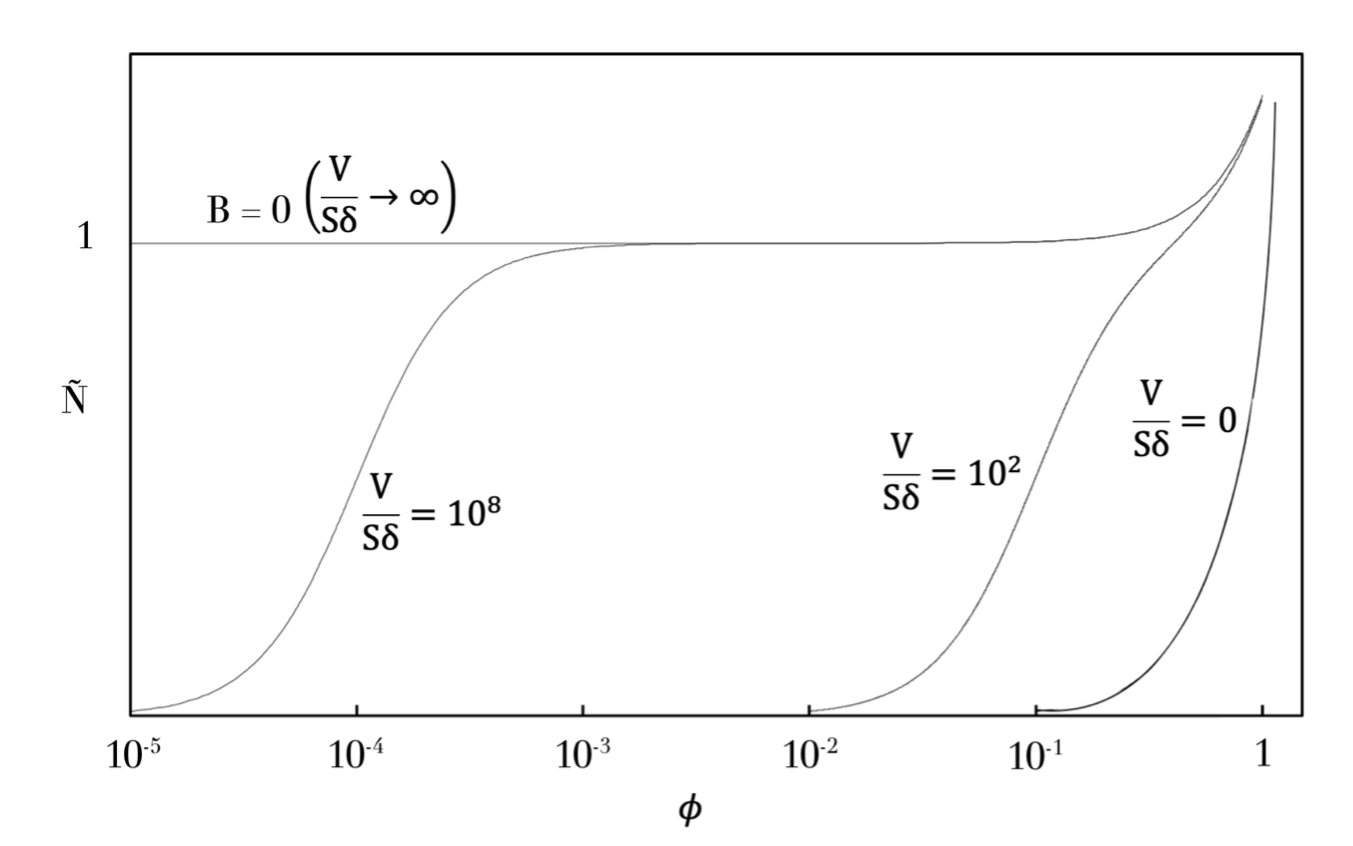
\includegraphics[width=\linewidth]{Capitulo2/Imagenes/Imagen_11_cap_2.png}
    \caption{Absorición de gas con reacción química}
    \label{fig:fig_2.11}
\end{figure}

La ecuación \eqref{eq_2.70} se grafica en la fig. \eqref{fig:fig_2.11}. Se puede observar en la fig. \eqref{fig:fig_2.11}:
\begin{enumerate}
    \item $\widetilde{N}$ aumenta con $\phi$ para todo $\frac{V}{S\delta}$
    \item $\widetilde{N}=1$ es la curva sin reacción que corresponde a la \eqref{fig:fig_2.10}. Cuando $\phi=0$ $\widetilde{N}\rightarrow1$ ($B=0$)
    \item Cuando $\phi\rightarrow0$, para $\frac{V}{S\delta}$ finito $\widetilde{N}=0$, se lidia con un líquido saturado con gas disuelto.
    \item Si $\phi$ es grande, $\widetilde{N}$ se incrementa abruptamente $(B\rightarrow 0)$ y la ec \eqref{eq_2.70} revela que $\widetilde{N}$ es proporcional a $\phi$. La reacción es muy rápida y el gas disuelto se consume dentro de la película. 
    \item Para valores intermedios de $\frac{V}{S\delta}$ y $\phi$, $\widetilde{N}\rightarrow1$. La reacción es rápida y la solución se encuentra libre de soluto. 

\end{enumerate}

\section{Difusión con reacción química heterogénea}

Considérese un reactor catalítico, en donde se lleva a cabo la reacción $2A\rightarrow B$, de acuerdo a la figura \eqref{fig:fig_2.12}

\begin{figure}[H]
    \centering
    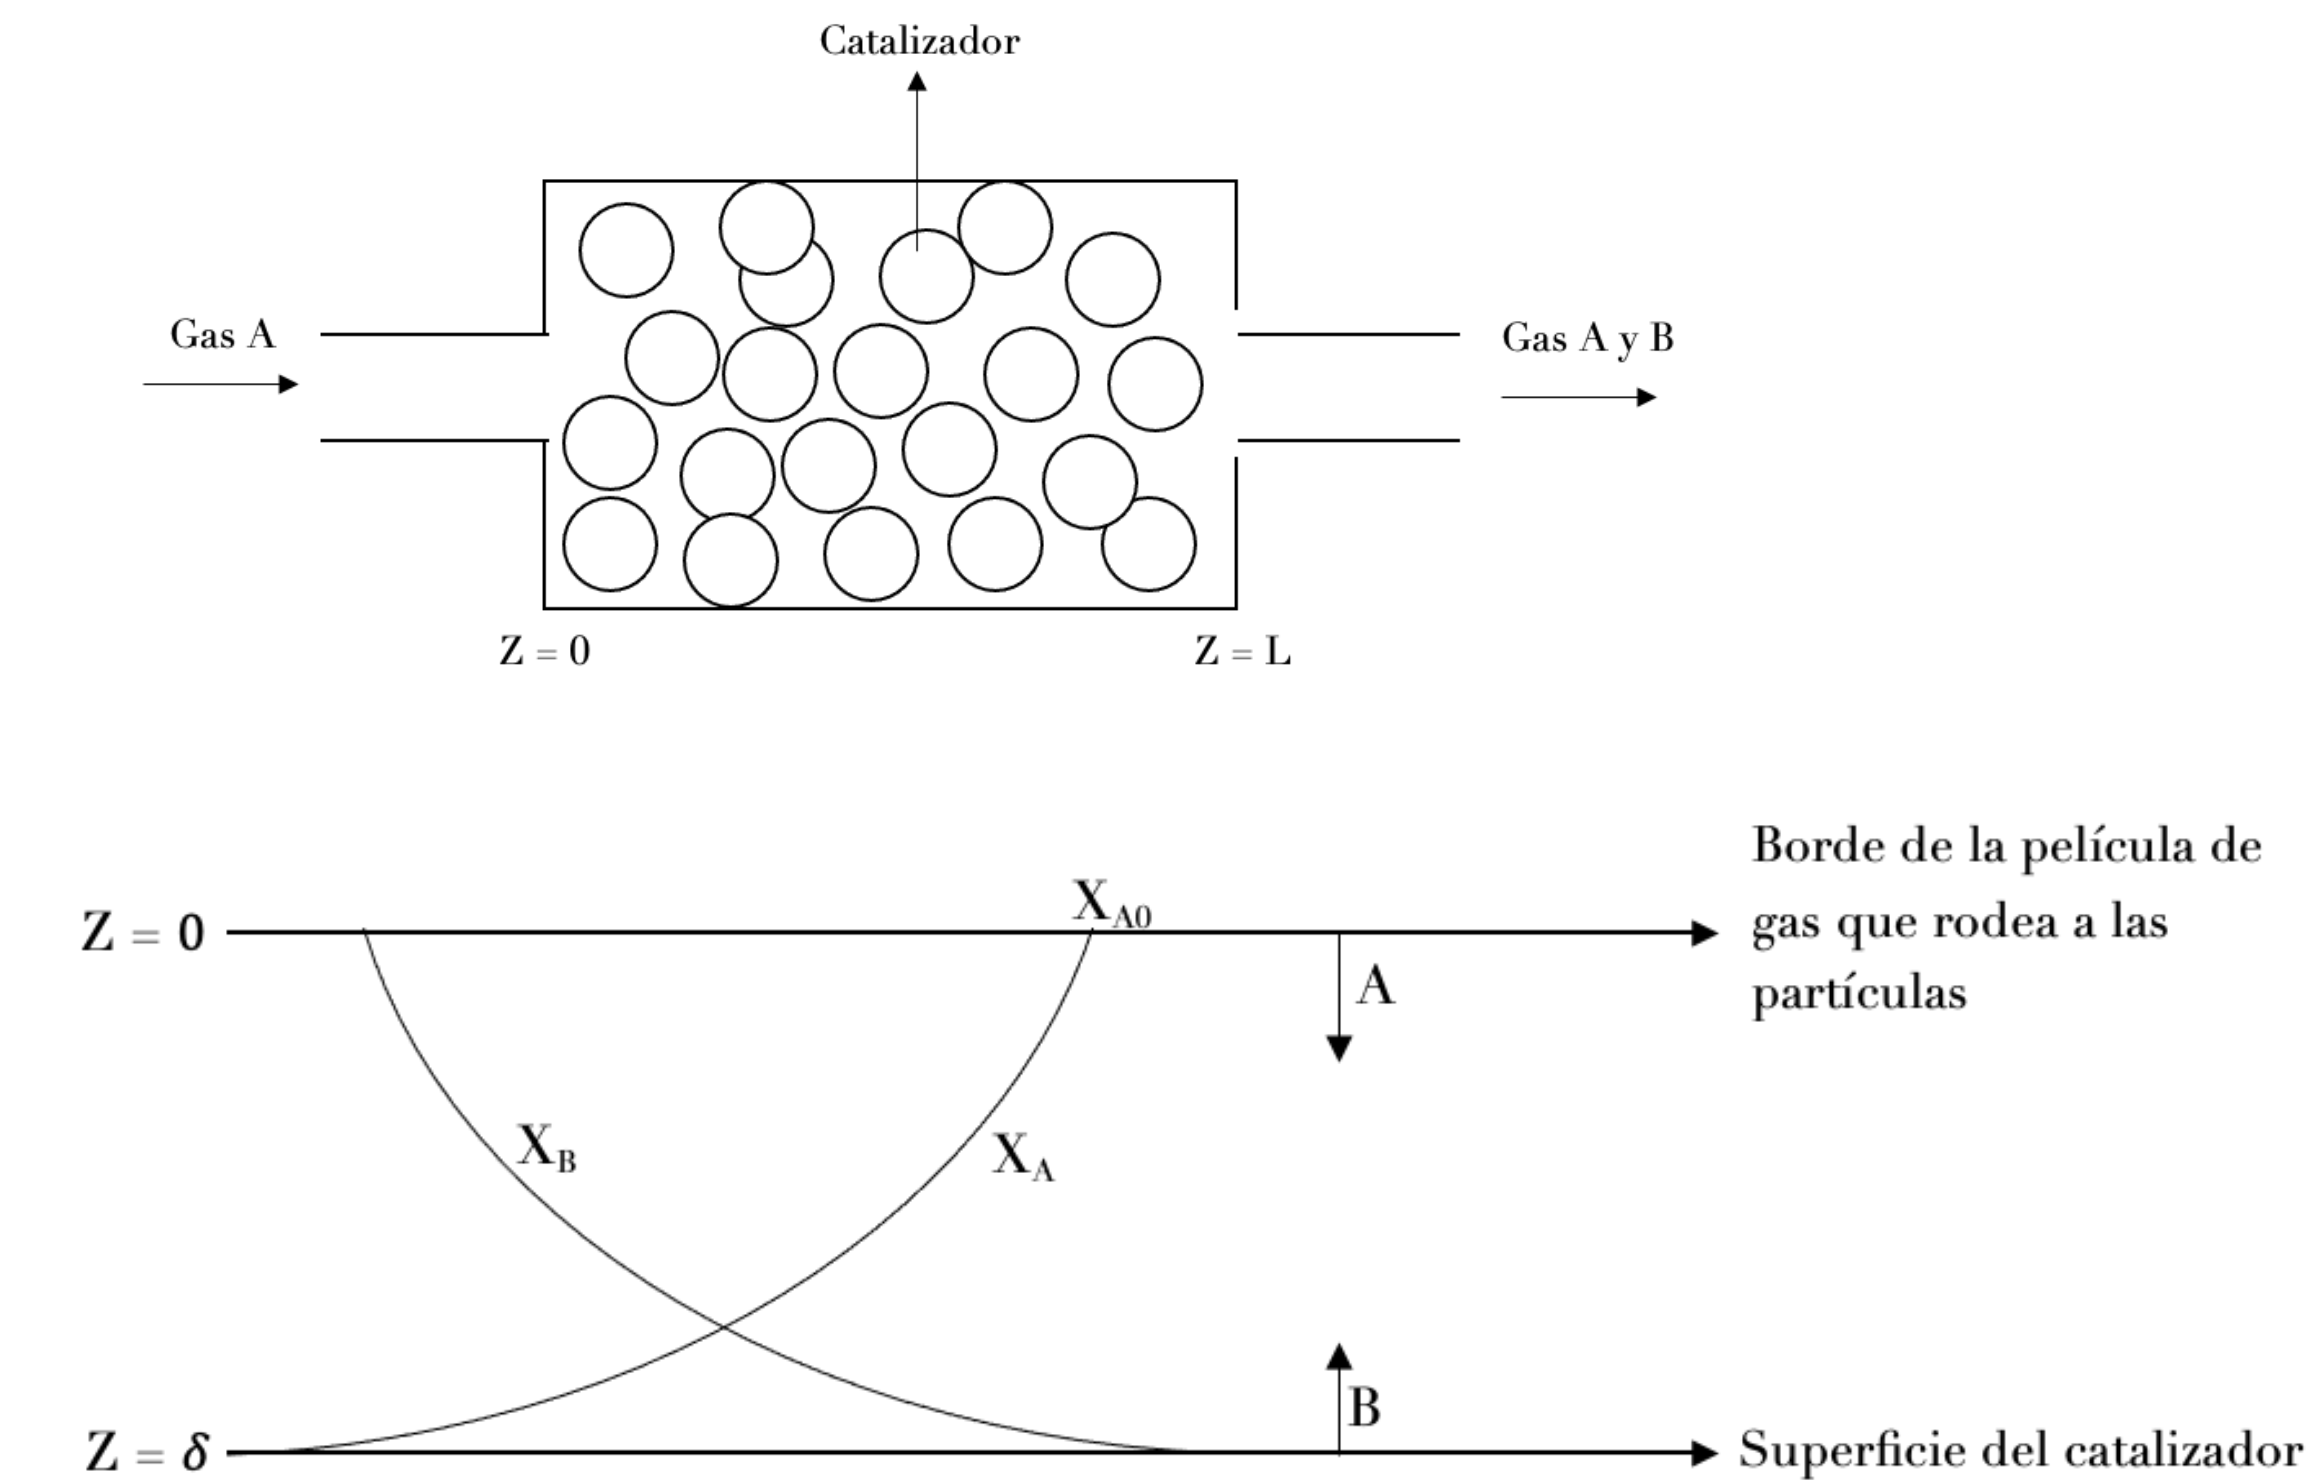
\includegraphics[width=\linewidth]{Capitulo2/Imagenes/Fig_2.12.png}
    \caption{Reactor catalítico en donde $2A\to B$\\Modelo de difusión cerca de la partícula de catalizador}
    \label{fig:fig_2.12}
\end{figure}

2 moles de A se mueven en dirección +z y un mol de B se mueve en dirección -z. Por lo tanto, a régimen permanente:

\begin{equation}
    N_{Bz}=-\frac{1}{2}N_{Az}
    \label{eq_2.71}
\end{equation}

Las ecs \eqref{eq_1.25} y \eqref{eq_1.19} en combinación con la ec \eqref{eq_2.71} son:

\begin{equation}
    N_{Az}=-\frac{c\mathscr{D}_{AB}}{1-\frac{x_A}{2}}\frac{d(x_A)}{dz}
\end{equation}
\begin{equation}
   \text{y} \quad \frac{d(N_A)}{dz}=0
\end{equation}


que resulta en:
\begin{equation}
    \frac{d}{dz}\left(\frac{1}{1-\frac{1}{2}x_A}\frac{dx_A}{dz}\right)=0
    \label{eq_2.74}
\end{equation}




Con las condiciones en la frontera:

\begin{equation}
    x_A |_{z=0} = x_{A0}\quad \text{y} \quad x_A |_{z=\delta} = 0
    \label{eq_2.75}
\end{equation}

A partir de la ec. \eqref{eq_2.74}, se obtiene:

\begin{equation*}
    \frac{1}{1-\frac{x_A}{2}}\frac{dx_A}{dz}=C_1\longrightarrow \int\frac{dx_A}{1-\frac{x_A}{2}}=C_1\int dz +C_2
\end{equation*}

Evaluando $C_1$ y $C_2$ con respecto a las condiciones \eqref{eq_2.75}, se obtiene:

\begin{equation}
    N_{Az}=\frac{2C\mathscr{D}_{AB}}{\delta}\ln\left(\frac{1}{1-\frac{1}{2}x_{A0}}\right)
    \label{eq_2.76}
\end{equation}

La reacción ocurre instantáneamente, por lo que la convección de A en B es un proceso controlado por difusión.

\subsection{Difusión con reacción heterogénea lenta}

En este caso, para el mismo sistema, la reacción no sucede instantáneamente en $z=\delta$, sino que la desaparición de A en la superficie del catalizador es proporcional a la concentración de A en la interfase:

\begin{equation}
    N_{Az}=k_1C_A=k_1Cx_A
\end{equation}

En este caso, la condición de frontera en la superficie del catalizador es:

\begin{equation*}
    x_A|_{z=\delta}=\frac{N_{Az}}{k_1c}
\end{equation*}

El cambio en la condición de frontera, resulta en el siguiente perfil:

\begin{equation}
    \frac{1-\frac{x_A}{2}}{(1-\frac{x_{A0}}{2})^{1-\frac{z}{\delta}}}=\left(1-\frac{N_{Az}}{2k_1c}\right)^{\frac{z}{\delta}}
\end{equation}



\begin{equation}
\begin{split}
     \frac{d}{dz}\ln\left(1-\frac{x_A}{2}\right)-\frac{d}{dz}\left[\left(1-\frac{z}{\delta}\right)\ln\left(1-\frac{x_{A0}}{2}\right)\right]=\frac{d}{dz}\left[\frac{z}{\delta}\ln \left(1-\frac{N_{Az}}{2k_1c}\right)\right]\\-\frac{\frac{1}{2}}{1-\frac{x_A}{2}}\frac{dx_A}{dz}+\frac{1}{\delta}\ln \left(1-\frac{x_{A0}}{2}\right)=\frac{1}{\delta}\ln \left(1-\frac{N_{Az}}{2k_1c}\right)   
\end{split}
\label{eq_2.79}
\end{equation}

Substituyendo la ec \eqref{eq_2.79} en la ec \eqref{eq_2.74}, se obtiene:

\begin{equation*}
    N_{Az}=-\frac{c\mathscr{D}_{AB}}{(1-\frac{x_A}{2})}\left[\left(1-\frac{x_A}{2}\right)\left(\frac{-2}{\delta}\right)\ln \left(\frac{1-\frac{N_{Az}}{k_1c}}{1-\frac{x_{A0}}{2}}\right)\right]
\end{equation*}
Aproximando $\ln (1-\frac{N_{Az}}{2k_1c})\approx -\frac{1}{2}\frac{N_{Az}}{k_1c}$, se obtiene:

\begin{equation*}
   N_{Az}=\frac{2C\mathscr{D}_{AB}}{\delta}\left[-\frac{N_{Az}}{2k_1c}-\ln \left(1-\frac{x_{A0}}{2}\right)\right] 
\end{equation*}
\begin{equation*}
   N_{Az}\left(1+\frac{\mathscr{D}_{AB}}{k_1\delta}\right)=2C\frac{\mathscr{D}_{AB}}{\delta}\ln \left(\frac{1}{1-\frac{1}{2}x_{A0}}\right)  
\end{equation*}
\begin{equation}
   N_{Az}=2c\frac{\mathscr{D}_{AB}}{\delta(1+\frac{\mathscr{D}_{AB}}{k_1\delta})}\ln \left(\frac{1}{1-\frac{1}{2}x_{A0}}\right)  
\end{equation}

El número adimensional $\frac{k_1\delta}{\mathscr{D}_{AB}}=Da$ es el número de Damköler, el cual describe la relación entre reacción y difusión. Si $Da\rightarrow\infty$, se obtiene el caso de reacción dominante y la ecuación toma la forma de la ec. \eqref{eq_2.76}

\section{Difusión con reacción química en medios porosos}

En este caso, se describe la difusión de los reactivos en un medio poroso en términos de una difusividad efectiva ($D_A$). Supóngase que la reacción tiene lugar en la superficie sólida de un catalizador cuya simetría es esférica y posee un radio R, la reacción es $A\rightarrow B$. Esta partícula esférica está sumergida en una corriente de gas con A y B presentes. A se difunde en los poros de la superficie esférica y ahí sucede la reacción. La ec \eqref{eq_1.30} dentro del medio poroso en coordenadas esfericas es:

\begin{equation}
    0=D_A\frac{1}{r^2}\frac{d}{dr}(r^2\frac{d(C_A)}{dr})-R_A
    \label{eq_2.81}
\end{equation}

"a" se define como la superficie catalítica por unidad de volumen (sólido + huecos). Por ello, $R_A=-k_1ac_a$.

Haciendo un cambio de variable, $\frac{C_A}{C_{AR}}=\frac{f(r)}{r}$ en donde $C_{AR}$ es la concentración de A en la superficie esférica, la ec \eqref{eq_2.81} se transforma en:

\begin{equation}
    \frac{d^2f}{dr^2}-\frac{k_1a}{D_A}f=0
    \label{eq_2.82}
\end{equation}

Con condiciones en la frontera:

\begin{equation}
    C_A|_{r=R}=C_{AR} \quad \text{y} \quad C_A|_{r=0}=finito
\end{equation}
o bien:
\begin{equation*}
    f|_{r=R}=R\quad \text{y} \quad
    f|_{r=0}=\text{finito}
\end{equation*}

La solución a la ecuación \eqref{eq_2.82} corresponde a:

\begin{equation}
    f(r)=C_1\cosh[(\frac{k_1a}{D_A})^\frac{1}{2}r]+C_2\sinh[(\frac{k_1a}{D_A})^\frac{1}{2}r]
\end{equation}
\begin{equation*}
    f(0)=C_1=0
\end{equation*}
\begin{equation*}
    f(R)=C_2\sinh[(\frac{k_1a}{D_A})^\frac{1}{2}R]=R\longrightarrow C_2=\frac{R}{sinh[(\frac{k_1a}{D_A})^\frac{1}{2}R]}
\end{equation*}

Por lo tanto:

\begin{equation}
    f(r)=\frac{R\sinh[(\frac{k_1a}{D_A})^\frac{1}{2}r]}{\sinh[(\frac{k_1a}{D_A})^\frac{1}{2}R]}
\end{equation}

Definiendo el modulo de Thiele como $\phi=\sqrt{\frac{k_1a}{D_A}}R$, entonces:
    $f(r)=\frac{R\sinh[\phi(\frac{r}{R})]}{\sinh\phi}$
Luego, 
\begin{equation}
    \frac{C_A}{C_{AR}}=\frac{R}{r}\frac{\sinh[\phi(\frac{r}{R})]}{\sinh\phi}
\end{equation}


Claramente, $\frac{C_A}{C_{AR}}|_{r=0}=\frac{\phi}{\sinh\phi}$ 
\newline
El flujo molar en la superficie es: $W_{AR}=4\pi R^2N_{AR}=-4\pi R^2D_A\frac{d(C_A)}{dr}|_{r=R}$
\begin{equation*}
\begin{split}
        \frac{d(C_A)}{dr}|_{r=R}=\frac{C_{AR}R}{\sinh \phi}\left[\frac{r}{r^2}\cosh\left[\frac{\phi r}{R}\right]\left(\frac{\phi}{R}\right)-\frac{1}{r^2}\sinh \left[\frac{\phi r}{R}\right]\right]\\
=\frac{C_{AR}R}{\sinh (\phi)}\left[\frac{\phi}{R^2}\cosh \phi-\frac{\sinh \phi}{R^2}\right]=\frac{C_{AR}}{R}[\phi \coth \phi-1]
\end{split}
\end{equation*}

Por lo tanto:

\begin{equation}
    W_{AR}=4\pi RC_{AR}D_A[1-\phi \coth (\phi)]
    \label{eq_2.87}
\end{equation}

Definiendo al factor de efectividad $\eta$:

\begin{equation}
    \eta=\frac{N_{AR}}{N_{AR0}}
    \label{eq_2.88}
\end{equation}
En donde $N_{AR0}$ es el flujo molar sin efectos difusionales, es decir:

\begin{equation}
    N_{AR0}=\frac{4\pi R^3}{3}a(-k_1C_{AR})
    \label{eq_2.89}
\end{equation}

Sustituyendo las ecs \eqref{eq_2.87} y \eqref{eq_2.89} en la ec \eqref{eq_2.88} resulta en: 

\begin{equation}
    \eta_A=\frac{3}{\phi^2}[\phi \coth (\phi)-1]
    \label{eq_2.90}
\end{equation}

Físicamente, $\eta_A$ es el factor tal que $\eta_AW_{AR0}$ representa la resistencia difusional del proceso. Para partículas no esféricas, el radio $R_{n e}$ se define como:

\begin{equation}
    R_{ne}=3\left(\frac{V_p}{S_p}\right)
\end{equation}

De tal forma que para partículas esféricas: $\frac{V_p}{S_p}=\frac{\frac{4\pi R^3}{3}}{4\pi R^2}=\frac{R}{3}$

En este caso, el valor de conversión absoluto en la reacción corresponde a:
\begin{equation*}
    |W_{AR}|=V_pak_1C_{AR}\eta_A
\end{equation*}
y donde ahora:
\begin{equation}
    \eta_A=\frac{1}{3\Lambda^2}(3\Lambda \coth 3\Lambda-1)
\end{equation} 
y
\begin{equation}
    \Lambda=(\frac{k_1a}{D_A})^{\frac{1}{2}}(\frac{V_p}{S_p})
\end{equation}
Es el modulo de Thiele generalizado. La variación de $\eta_A$ en función de $\Lambda$ se grafica en la fig \eqref{fig:fig_2.13} para diferentes geometrías

\begin{figure}[H]
    \centering
    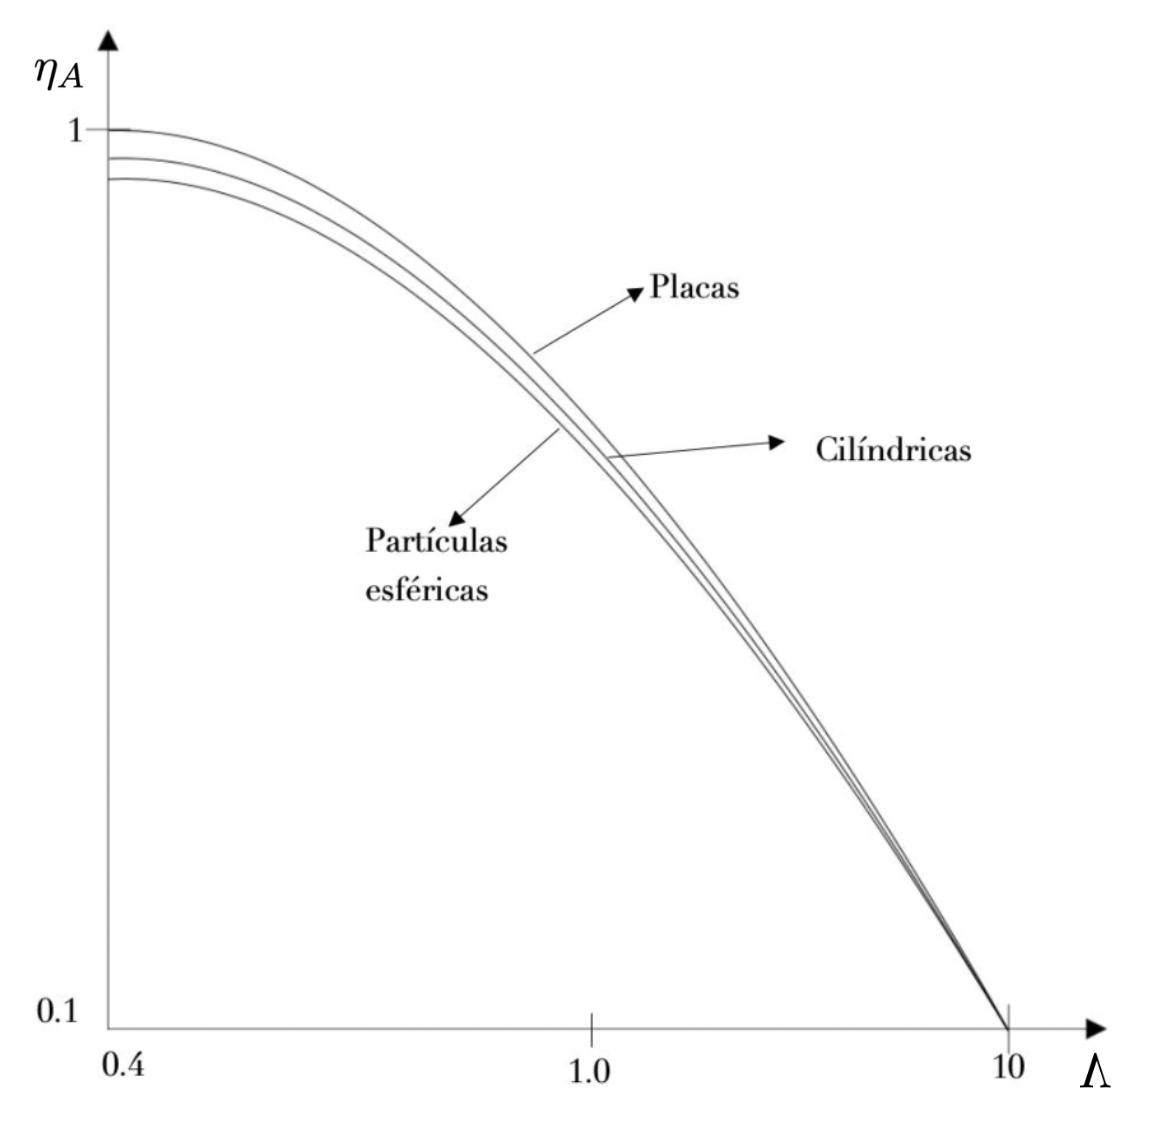
\includegraphics[width=0.7\linewidth]{Capitulo2/Imagenes/Fig_2.13.png}
    \caption{Factores de efectividad en catalizadores porosos de varias fromas}
    \label{fig:fig_2.13}
\end{figure}
\newpage
\section*{Apéndice A}
\renewcommand{\thefigure}{A.\arabic{figure}}
\setcounter{figure}{0}
\renewcommand{\theequation}{A.\arabic{equation}} 
\setcounter{equation}{0}
Difusión debido a una fuente puntual en una corriente de fluído.
Un fluido B fluye a una velocidad constante $v_0$. en algún punto, la especie A se inyecta a un flujo $W_A$ (gmol/s) que es suficientemente pequeño. A se difunde axial y radialmente.

Como este es un problema de convección-difusión, en coordenadas cilíndricas (vea la ec. \eqref{eq_B} en el apéndice B), en la dirección z, se tiene:

\begin{equation}
    \frac{\partial C_A}{\partial t}+v_z\frac{\partial C_A}{\partial z}=\mathscr{D}_{AB}\left[\frac{1}{r}\frac{\partial }{\partial r}\left(r\frac{\partial C_A}{\partial r}\right)+\frac{\partial ^2C_A}{\partial z^2}\right]
\end{equation}
en donde $dt=\frac{dz}{v_0}$.

Ahora, se realiza un cambio de variable $C_A(r,z)=C_A(s,z)$, en la cual $s^2=r^2+z^2$ (ver fig. \eqref{fig:Fig_A.1.})
\begin{figure}[H]
    \centering
    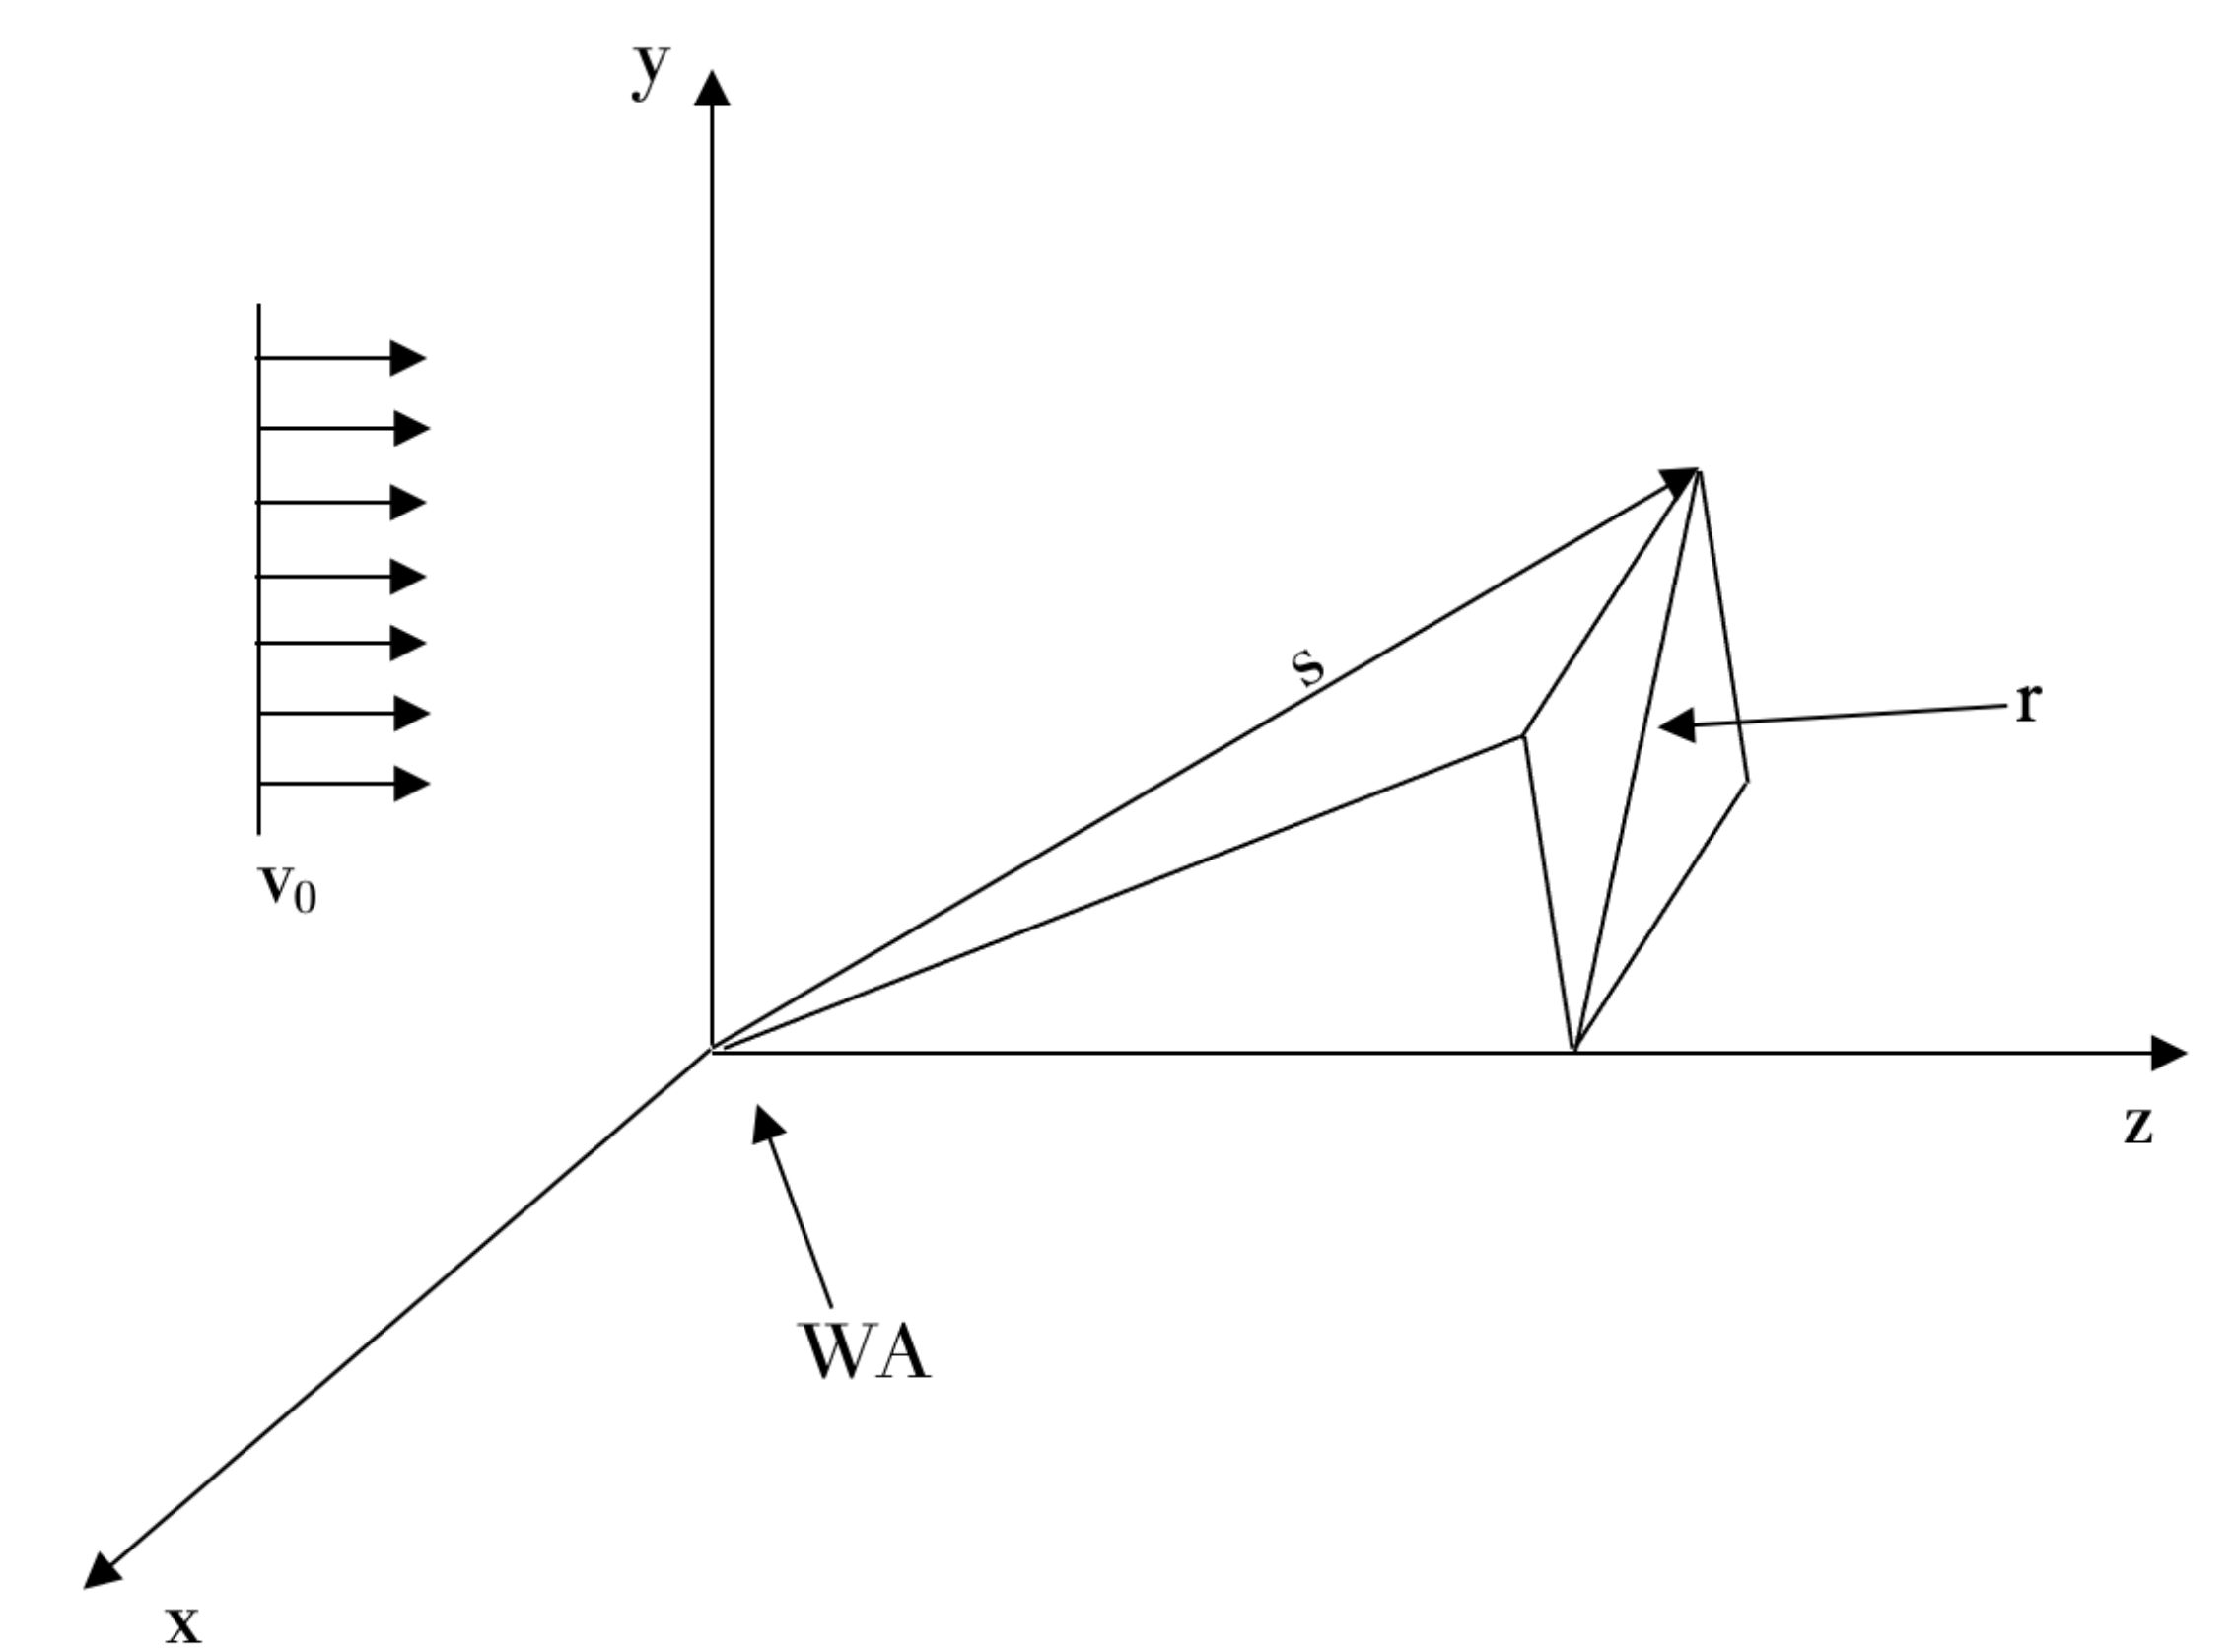
\includegraphics[width=0.5\linewidth]{Capitulo2/Imagenes/Fig_A.1.png}
    \caption{Difusión de A desde una fuente puntual en una corriente de B que va a una velocidad $v_0$ constante}
    \label{fig:Fig_A.1.}
\end{figure}

El diferencial $dC_A$ por regla de la cadena, corresponde a:

\begin{equation*}
    dC_A=(\frac{\partial C_A}{\partial s})_zds+(\frac{\partial C_A}{\partial z})_sdz
\end{equation*}
Luego:
\begin{equation*}
    (\frac{\partial C_A}{\partial z})_r=(\frac{\partial C_A}{\partial s})_z\frac{ds}{dz}+(\frac{\partial C_A}{\partial z})_s
\end{equation*}
Recordando que $s^2=r^2+z^2$, por lo tanto, $\frac{\partial s}{\partial z}=\frac{z}{s}$
\begin{equation*}
    (\frac{\partial C_A}{\partial z})_r=(\frac{\partial C_A}{\partial s})_z\frac{z}{s}+(\frac{\partial C_A}{\partial z})_s
\end{equation*}

\begin{equation*}
    (\frac{\partial^2C_A}{\partial z^2})_r=\frac{\partial}{\partial z}((\frac{dC_A}{dz})_r)
\end{equation*}
\begin{equation*}
    (\frac{\partial^2C_A}{\partial z^2})_r=[\frac{\partial}{\partial s}((\frac{\partial C_A}{\partial s})_r)\frac{\partial s}{\partial z}+\frac{\partial }{\partial z}((\frac{\partial C_A}{\partial s})_r)]_s
\end{equation*}
\begin{equation*}
    (\frac{\partial^2C_A}{\partial z^2})_r=\frac{\partial}{\partial s}[(\frac{\partial C_A}{\partial s})_z\frac{z}{s}+(\frac{\partial C_A}{\partial z})_s]\frac{z}{s}+\frac{\partial }{\partial z}[(\frac{\partial C_A}{\partial s})_z\frac{z}{s}+(\frac{\partial C_A}{\partial z})_s]
\end{equation*}
\begin{equation*}
    (\frac{\partial^2C_A}{\partial z^2})_r=\frac{z}{s}[(\frac{\partial^2 C_A}{\partial s^2})_z\frac{z}{s}-(\frac{\partial C_A}{\partial s})_z\frac{z}{s^2}+\frac{\partial^2C_A}{\partial s \partial z}]
\end{equation*}
\begin{equation*}
    +[(\frac{\partial^2C_A}{\partial z \partial s})\frac{z}{s}+(\frac{\partial C_A}{\partial s})_s\frac{1}{s}+(\frac{\partial^2C_A}{\partial z^2})_s]
\end{equation*}
Se calculan ahora, las derivadas radiales:

\begin{equation*}
    (\frac{\partial C_A}{\partial r})_z=(\frac{\partial C_A}{\partial s})_z(\frac{\partial s}{\partial r})_z=(\frac{\partial C_A}{\partial s})_z(\frac{r}{s})=(\frac{\partial C_A}{\partial s})_z(\frac{(s^2-z^2)^\frac{1}{2}}{s})
\end{equation*}
\begin{equation*}
     r(\frac{\partial C_A}{\partial r})_z=(\frac{\partial C_A}{\partial s})_z(\frac{s^2-z^2}{s})
\end{equation*}
\begin{equation*}
    \frac{1}{r}\frac{\partial}{\partial r}(r(\frac{\partial C_A}{\partial r})_z)=\frac{1}{s}\frac{\partial}{\partial s}[(\frac{s^2-z^2}{s})(\frac{\partial C_A}{\partial s})_z]
\end{equation*}
\begin{equation*}
    =\frac{1}{s}[(\frac{s^2-z^2}{s})(\frac{\partial C_A}{\partial s})_z]+(\frac{s^2-z^2}{s})(\frac{\partial^2C_A}{\partial s^2})_z
\end{equation*}

Sumando, se obtiene:
\begin{equation*}
    \frac{\partial^2C_A}{\partial z^2}+2\frac{z}{s}\frac{\partial^2C_A}{\partial s \partial z}+\frac{\partial^2C_A}{\partial s^2}+\frac{z}{s}(\frac{\partial C_A}{\partial s})
\end{equation*}
O de manera equivalente:
\begin{equation*}
    \frac{\partial^2C_A}{\partial z^2}+2\frac{z}{s}\frac{\partial^2C_A}{\partial s \partial z}+\frac{1}{s^2}\frac{\partial}{\partial s}(s^2\frac{\partial C_A}{\partial s})=f(s,r,z)
\end{equation*}
Al insertar en la ecuación (A.1), se obtiene:
\begin{equation*}
    v_0(\frac{z}{s}\frac{\partial C_A}{\partial s}+\frac{\partial C_A}{\partial z})=\mathscr{D}_{AB}f(s,r,z)
\end{equation*}
Cuya solución es:
\begin{equation}
    C_A=[\frac{W_A}{4\pi \mathscr{D}_{AB}s}]e^{\frac{-v_0(s-z)}{2\mathscr{D}_{AB}}}
\end{equation}
Que satisface las condiciones de frontera:
\begin{equation*}
    1) C_A|_{z \rightarrow \infty}=0 
\end{equation*}
La concentración de A lejos de la fuente es 0
\begin{equation*}
    2) -\frac{\partial C_A}{\partial s}|_{s \rightarrow0}=\frac{W_A}{4\pi \mathscr{D}_{AB}s^2}
\end{equation*}
Este corresponde al sitio de la fuente
\begin{equation*}
    \frac{\partial C_A}{\partial s}=\frac{\partial}{\partial s}[\frac{a}{s}e^{b(s-z)}]=a[\frac{b}{s}e^{b(s-z)}-\frac{1}{s^2}e^{b(s-z)}]=ae^{b(s-z)}[\frac{b}{s}-\frac{1}{s^2}]
\end{equation*}
En donde $a=\frac{W_A}{4\pi \mathscr{D}_{AB}}$, entonces. Si $s\rightarrow 0$, recordando que $s^2=z^2+r^2$, tanto r como z deben tender a 0, por lo tanto:
\begin{equation*}
    \frac{\partial C_A}{\partial s}|_{s\rightarrow 0}=\quad\lim_{s\rightarrow0}ae^{b(s-z)}[\frac{b}{s}-\frac{1}{s^2}]
\end{equation*}
Se toma la siguiente consideración, en el límite $\frac{1}{s^2}>>\frac{b}{s}$ y $e^{b(s-z)=1}$. Por lo tanto:
\begin{equation*}
     \frac{\partial C_A}{\partial s}|_{s\rightarrow 0}=a(-\frac{1}{s^2})
\end{equation*}
y finalmente:
\begin{equation*}
   -\frac{\partial C_A}{\partial s}|_{s\rightarrow 0}=\frac{W_A}{4\pi \mathscr{D}_{AB}s^2} 
\end{equation*}
 \begin{equation*}
     3) \frac{\partial C_A}{\partial r}|_{r\rightarrow0}=0
 \end{equation*}
 Lo cual implica que la concentración máxima está en el eje z
 \begin{equation*}
    \frac{\partial C_A}{\partial r}=\frac{\partial C_A}{\partial s}\frac{\partial s}{\partial r}=\frac{r}{s}\frac{\partial C_A}{\partial s}=\frac{r}{s}(ae^{b(s-z)}[\frac{b}{s}-\frac{1}{s^2}])
 \end{equation*}
 si $r\rightarrow0$, $s\rightarrow z$ y el valor de la derivada es igual a 0, lo que nos dice que el máximo de la función $C_A$ está en el eje z.
 A partir de datos de $v_0$ y $W_A$ dados, se puede plantear un modelo de regresión lineal para la determinación de $\mathscr{D}_{AB}$.
 \begin{equation*}
     ln(C_As)=ln(\frac{W_A}{4\pi \mathscr{D}_{AB}})-v_0\frac{(s-z)}{2\mathscr{D}_{AB}}
 \end{equation*}
 En donde $s-z$ es la variable independiente y $C_{AS}$ la variable dependiente.

\begin{figure}[H]
    \centering
    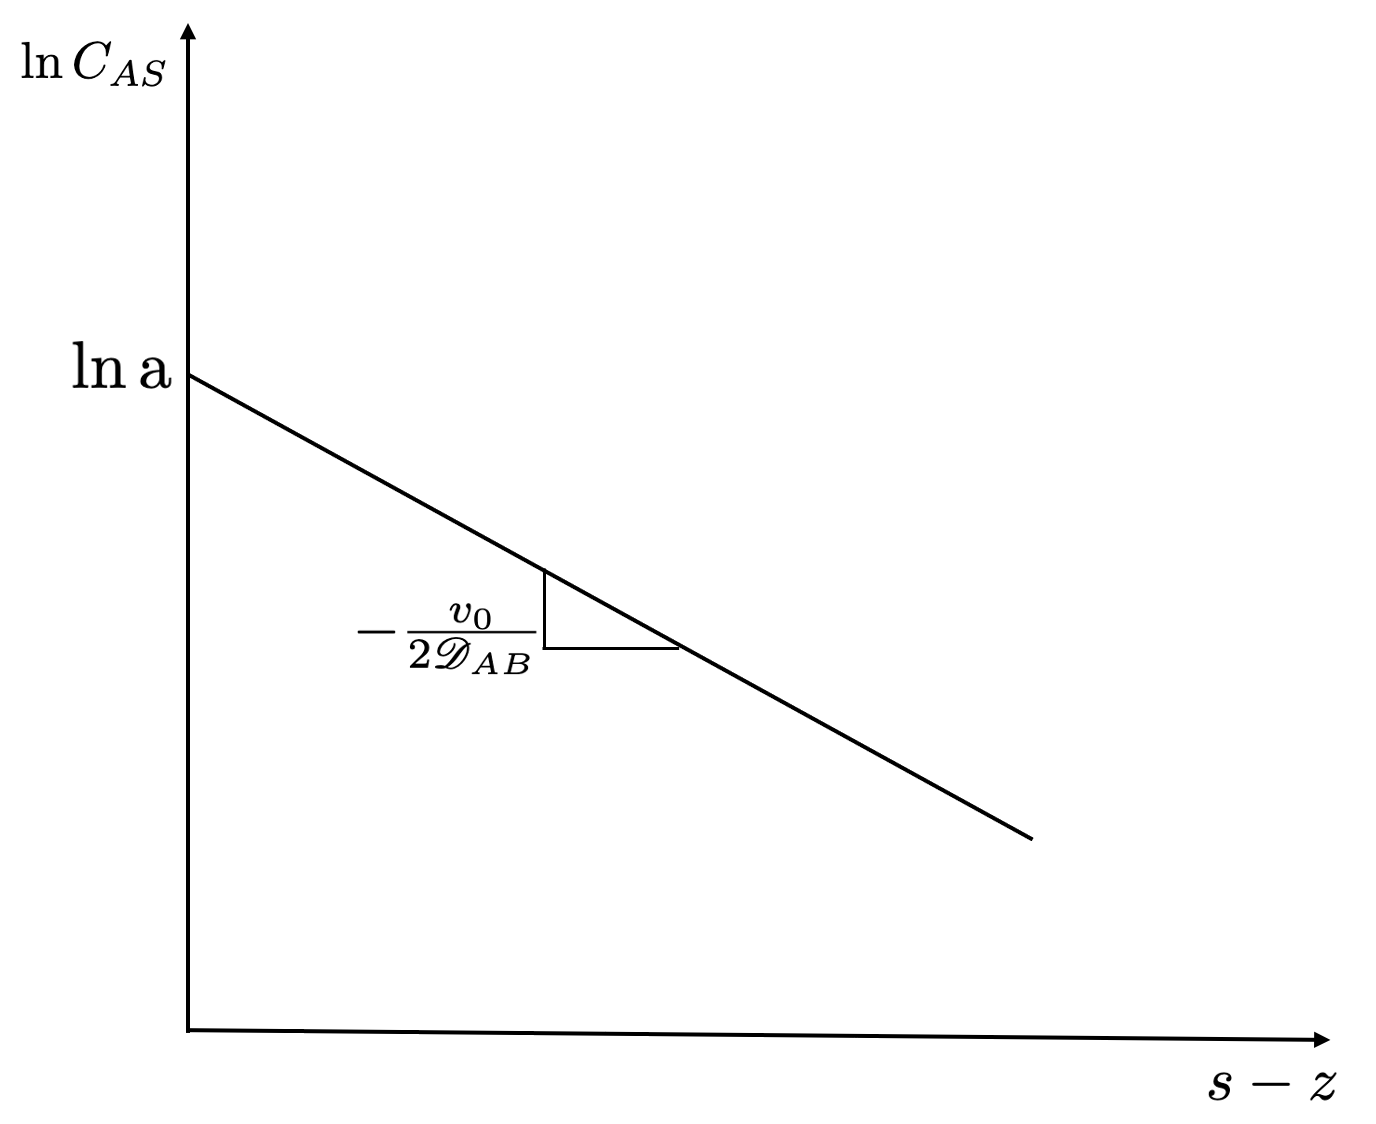
\includegraphics[width=0.5\linewidth]{Capitulo2/Fig_A2.png}
\end{figure}
 
